\documentclass[runningheads]{llncs}
%---- Sonderzeichen-------%
\usepackage[ngerman]{babel}
%---- Codierung----%
\usepackage[utf8]{inputenc}
%\usepackage[latin1]{inputenc}
\usepackage[T1]{fontenc}
\usepackage{graphicx}
\usepackage{url}
\usepackage{llncsdoc}
%----- Mathematischer Zeichenvorrat---%
\usepackage{amsmath}
\usepackage{amssymb}
\usepackage{enumerate}
% fuer die aktuelle Zeit
\usepackage{listings}
\usepackage{textcomp}
\usepackage{color}
\usepackage{subfigure}
\usepackage{hyperref}
\numberwithin{figure}{section}

\usepackage[citestyle=numeric,style=numeric,backend=biber]{biblatex}
\addbibresource{literature.bib}

%
% ECMAScript 2015 (ES6) definition by Gary Hammock
%

\lstdefinelanguage[ECMAScript2015]{JavaScript}[]{JavaScript}{
  morekeywords=[1]{await, async, case, catch, class, const, default, do,
    enum, export, extends, finally, from, implements, import, instanceof,
    let, static, super, switch, throw, try},
  morestring=[b]` % Interpolation strings.
}


%
% JavaScript version 1.1 by Gary Hammock
%
% Reference:
%   B. Eich and C. Rand Mckinney, "JavaScript Language Specification
%     (Preliminary Draft)", JavaScript 1.1.  1996-11-18.  [Online]
%     http://hepunx.rl.ac.uk/~adye/jsspec11/titlepg2.htm
%

\lstdefinelanguage{JavaScript}{
  morekeywords=[1]{break, continue, delete, else, for, function, if, in,
    new, return, this, typeof, var, void, while, with},
  % Literals, primitive types, and reference types.
  morekeywords=[2]{false, null, true, boolean, number, undefined,
    Array, Boolean, Date, Math, Number, String, Object},
  % Built-ins.
  morekeywords=[3]{eval, parseInt, parseFloat, escape, unescape},
  sensitive,
  morecomment=[s]{/*}{*/},
  morecomment=[l]//,
  morecomment=[s]{/**}{*/}, % JavaDoc style comments
  morestring=[b]',
  morestring=[b]"
}[keywords, comments, strings]


\lstalias[]{ES6}[ECMAScript2015]{JavaScript}

% Requires package: color.
\definecolor{mediumgray}{rgb}{0.3, 0.4, 0.4}
\definecolor{mediumblue}{rgb}{0.0, 0.0, 0.8}
\definecolor{forestgreen}{rgb}{0.13, 0.55, 0.13}
\definecolor{darkviolet}{rgb}{0.58, 0.0, 0.83}
\definecolor{royalblue}{rgb}{0.25, 0.41, 0.88}
\definecolor{crimson}{rgb}{0.86, 0.8, 0.24}

\lstdefinestyle{JSES6Base}{
  backgroundcolor=\color{white},
  basicstyle=\ttfamily,
  breakatwhitespace=false,
  breaklines=false,
  captionpos=b,
  columns=fullflexible,
  commentstyle=\color{mediumgray}\upshape,
  emph={},
  emphstyle=\color{crimson},
  extendedchars=true,  % requires inputenc
  fontadjust=true,
  frame=single,
  identifierstyle=\color{black},
  keepspaces=true,
  keywordstyle=\color{mediumblue},
  keywordstyle={[2]\color{darkviolet}},
  keywordstyle={[3]\color{royalblue}},
  numbers=left,
  numbersep=5pt,
  numberstyle=\tiny\color{black},
  rulecolor=\color{black},
  showlines=true,
  showspaces=false,
  showstringspaces=false,
  showtabs=false,
  stringstyle=\color{forestgreen},
  tabsize=2,
  title=\lstname,
  upquote=true  % requires textcomp
}

\lstdefinestyle{JavaScript}{
  language=JavaScript,
  style=JSES6Base
}
\lstdefinestyle{ES6}{
  language=ES6,
  style=JSES6Base
}
\renewcommand{\labelitemi}{$\bullet$}
%\renewcommand{\thefigure}{\thesection-\arabic{figure}}

\setcounter{tocdepth}{3}
\setcounter{secnumdepth}{3}

% -------------------------------------------------------------------------------------------------
% -------------------------------------------------------------------------------------------------
\mainmatter
\title{5G Edge Cloud Architektur}
\titlerunning{5G Edge Cloud Architektur}
\author{Julian Beck}
\authorrunning{Julian Beck}
\institute{Betreuer: Prof. Dr. rer. nat. Oliver Waldhorst}
\date{01.05.2019}
\begin{document}
\let\oldaddcontentsline\addcontentsline
\def\addcontentsline#1#2#3{}
\maketitle
\def\addcontentsline#1#2#3{\oldaddcontentsline{#1}{#2}{#3}}


% -------------------------------------------------------------------------------------------------

\begin{abstract}
  Die Edge Cloud wird in dem Zeitalter von 5G eine wichtige Rolle spielen. 
  Als ein Bestandteil der 5G-Netzwerkarchitektur bietet es nicht nur eine Vielzahl von Cloud-Ressourcen, sondern
  ermöglicht neue Platformen für Drittanbieter und das Entwickeln von neuen Erfahrungen für den Nutzer.
  Multi-Access Edge Computing (MEC) bietet Speicher- und Rechenressourcen in der Nähe des Endgerätes, 
  eine besser Latenzzeit für mobile Endbenutzer und effizientere Nutzung des Mobile Backhaul
  und Core Netzwerkes. Diese Seminararbeit erläutert, welche Technologien MEC ermöglicht und geht auf die Architekturen 
  hinter Multi-Access Edge Computing ein.
\end{abstract}

% -------------------------------------------------------------------------------------------------
\tableofcontents 
\newpage
% -------------------------------------------------------------------------------------------------

\section{Einleitung}
\label{sec:Einleitung}
In den letzten zehn Jahren haben Fortschritte im Cloud-Computing einen zentralisierten Ansatz für die Systemadministration und den 
Systembetrieb verfolgt, während das Wachstum von Mobile Computing, 
SaaS und dem Internet der Dinge (IoT) das Computing in Richtung einer verteilten Architektur in der Nähe des Anwenders getrieben hat. 
Mit der Einführung von 5G-und Edge-Computing-Technologien werden beide Ansätze kombiniert.
\\
\\
5G und Edge Computing sind zwei relativ neue Technologien, die aber ähnliche Ziele verfolgen. 
Beide sind darauf ausgerichtet, die Leistung von Anwendungen zu verbessern 
und die Verarbeitung von großer Datenmengen in Echtzeit zu ermöglichen. 
5G erhöht die Geschwindigkeit um das Zehnfache gegenüber 4G, 
während  Edge Computing die Latenz verringert, indem Rechenfunktionen näher am Endbenutzer in das Netzwerk integriert werden.
\\
\\
Während Telekommunikationsbetreiber berichten, 
dass 5G im Netzwerkgeschwindigkeiten erhöht
spiegelt dies nicht die Erfahrung eines durchschnittlichen Benutzers wieder. 
Die Edge Cloud kommt an dieser stelle ins Spiel und verbessert die Latenz und 
damit auch die Anwendungsmöglichkeiten von 5G.
Gleichzeitig benötigt 5G das Edge Computing, um die Nachfrage zu erhöhen und somit den Ausbau zu beschleunigen
\subsection{Problem}
\label{subsec:Problem}
5G Edge Computing bietet sich für folgende Anwendungen an:
\begin{itemize}
  \item Caching von Anwendungen und Videos
  \item Rechenressourcen an die Aufgaben übergeben werden können um möbile Endgeräte zu entlasten
  \item Bearbeitung und Aggregierung von IoT Daten.
  \item Rendern von Videospielen auf der EDGE Cloud.
\end{itemize}
Die Anwendungsbeispiele werden in Kaptiel \ref{sec:Anwendungen} genauer erläutert.
\newpage



\section{Benötigte Technologien}
\label{sec:Benötigte Technologien}
Dieses Kapitel bietet eine kurze Einführung in die Kerntechnologien die die Anwendung eines 5G Netzwerkes erforderlich sind.
\subsection{Edge Computing}
\label{sub:Edge Computing}
Bei Cloud-Computing werden Rechenressourcen über ein Netzwerk zur Verfügung gestellt.
Beim Edge Computing wird die Berechnung und Speicherung von Daten in die Nähe der Quelle gebracht,
an den sogenannten Rand oder \textit{Edge} des Netzwerks. Im Gegensatz zum Cloud Computing werden die Daten
nicht an zentralen Rechenzentren verarbeitet, sonden an dezentralen Cloud Systemen am Rand des Neztwerks. 
Folgende Vorteile bringt Edge Computing: \cite{labrieTopBenefitsEdge}
\begin{itemize}
  \item \textbf{Geschwindigkeit und Latenz:} Abhängig von der Anwendungen spielt die Zeit der Datenverarbeitung eine
  entscheidende Rolle. Beispielsweise bei Autonomen Fahrzeugen ist es wichtig, dass innerhalb von Millisekunden die Daten
  verarbeitet werden. Auch bei digitalen Fabriken ist es meist zu langsam die Daten zu einer zentralen Cloud und zurück
  zu senden. 
  Wenn die Datenverarbeitung auf den Rand des Netzwerks verlegt wird, wird die Latenz des Netzwerks verringert und schneller
  auf Anfragen geantwortet.
  \item \textbf{Netzlast:} Da das die Daten nicht zu einer zentralen Cloud gesendet werden, sonder am Rand des Netzwerks 
  verarbeitet werden, verringert sich nicht nur die Latenz, sondern auch die Netzlast des gesamten Netzwerks. 
  Die Daten müssen nicht weitreichend weiter gesendet werden, stattdessen werden sie 
  dezentral in der Nähe der Anwendungen verarbeitet.
  \item \textbf{Security:} Wenn Daten an einem zentralen Cloud verarbietet werden ist dies unter bestimmten Umständen anfälliger
  für ein Ausfall.
  So kann beispielsweise ein DDoS-Angriff den gesammten Betrieb eines Unternehmens stören, wenn alle Systeme mit einer zentralen
  Cloud arbeiten. Da bei Edge Computing kein einziges Zentrales Systeme existiert, verringert sich die Auswirkung eines solchen
  Angriffes für das ganze Unternehmen.  
  Edge Computing hilft Unternehmen auch dabei, die Probleme der lokalen Compliance- und Datenschutzbestimmungen zu überwinden,
  da die Daten auf lokalen Systemen verarbeitet werden.
  \item \textbf{Kosteneinsparungen:} Durch Internet Off Things Geräte oder durch eine Smart Factories werden
  eine Vielzahl an Daten generiert. Nicht alle Daten sind dabei kritisch für die Operation der Systeme. Edge Computing erlaubt
  das Kategorisieren der Daten. In dem ein Großteil der Verarbeitung am Rand des Netzwerks stattfindet wird Bandbreite gespart.
  Dies optimiert den Datenfluss von lokalen Anwendungen und minimiert somit die Betriebskosten einer zentralen Cloud.
  \item \textbf{Zuverlässigkeit:} Wenn Edge-Geräte Daten lokal speichern und verarbeiten können, verbessert dies die Zuverlässigkeit.
  Ein Unternehmen ist nicht auf die Verbindung auf zur zentralen Cloud angewiesen und eine eine vorübergehende Unterbrechungen der 
  Verbingung hat keine Auswirkungen auf den Betrieb von Geräte, nur weil sie die Verbindung zur Cloud verloren haben.
  \item \textbf{Skalierbarkeit:}
  Bei Cloud-Computing-Architekturen müssen Daten in den meisten Fällen zunächst an ein zentral gelegenes Rechenzentrum
  weitergeleitet werden. Das Erweitern oder sogar nur das Ändern dedizierter Rechenzentren ist eine teure Angelegenheit. 
  Darüber hinaus können IoT-Geräte zusammen mit ihren Verarbeitungs- und Datenverwaltungstools am Rande einer einzelnen 
  Implantation bereitgestellt werden, 
  anstatt auf die Koordination der Bemühungen von Mitarbeitern an mehreren Standorten zu warten.

\end{itemize}
\newpage
\subsection{5G Network}
\label{subsec:5G Network}
Das 5G-Netzwerk wurde  entwickelt, um Dienste zu unterstützen, 
die eine Verwendung durch die Industrie mithilfe Techniken wie 
Netzwekrsfunktions Virtualisierung und Software Defined Networking ermöglicht.
Klassischerweise wurden mobile Netzwere in erster Linie für den Smartphone Geräte konzeptiert. 
Dies ändert sich bei dem 5G Netzwerk, durch eine Vielzahl von Anwendungen und unterschiedliche Datenanforderungen,
muss das Netzwerk so konzeptiert sein um alle diese Anforderungen zu erfüllen.
\\
\\
Bei der 5G Architektur sind die Netzwerkfunktionen der Control Plane (CP) von der User Plane (UP) getrennt, 
um diese unabhängig skalieren zu können. Dies ermöglichen Netzwerkbetreiber das Anpassen und Skalieren des Neztwerks an die
benötigten Anforderungen.
\\
\\
Die Darstellung zeigt die einzelnen Komponenten in Form einer Service basierten Darstellung.  \cite{5GCoreNetwork2017}
Das 5G Netzwerk besteht aus sogenannten Netzwerkfunktionen, die meist softwarebasiert sind und so nach Bedarf angepasst/skaliert werden können.
Die 5G CP ist das Kernnetz, dass aus einer Reihe von Netzwerkfunktionen besteht, 
die für die Separierung, Priorisierung und Zugriffssteuerung erforderlich sind:
\begin{itemize}
  \item \textbf{Authentication Server Function (AUSF)} dient als Authentifizierungsserver
  \item \textbf{Core Access and Mobility Management Function (AMF)} ist für die Integrität, Registrierungsmanagement, Verbindungsmanagement,
  Zugriffs und Securitymanagement zuständig
  \item \textbf{Network Exposure Function (NEF)} verbreiten von Funktionen und Events, 
  sichere Bereitstellung von Informationen aus externen Anwendungen für das 3GPP-Netzwerk. Diese Funktion ist vorallem für die Mobilität
  in der 5G Edge Cloud wichtig, was in Abschnitt \ref{subsec:MEC Mobilität} erläutert wird.
  \item \textbf{Session Management Function (SMF)} Sitzungsverwaltung, Zuweisung von IP Adressen an die Endgeräte. 
  \item \textbf{Unified Data Management (UDM)} Generierung von Anmeldeinformationen für Authentifizierungen, 
  Verwalten der Benutzeridentifikation und Zugriffsautorisierung.
  \item \textbf{User plane Function (UPF)} Datenrouting und Weiterleitung. Dateninspektionen.
  \item \textbf{Policy Control function (PCF)} Bereitstellung von Richtlinien für Funktionen, 
  Zugriff auf Abonnementinformationen
\end{itemize}
\subsection{5G Edge Computing}
\label{subsec:5G Edge Computing}
\subsection{Netzwekrsfunktions Virtualisierung}
\label{subsec:Netzwekrsfunktions Virtualisierung}
Netzwekrsfunktions Virtualisierung (NFV) erlaubt es Netzwerkfunktionen, von der Hardware zu entkoppeln.
Dies ermöglicht das Verwenden von Gateways, Firewalls, DNS Services und Caching ohne proprietär Hardware.
\\
\\
Um ein neues Netwzerk zu erstellen, wird eine Vielzahl von verschieden Hardware Komponenten benötigt. 
Diese benötigen Platz, Energy und müssen von qualifizierten Personal überwacht und gewartet werden. 
Netzwekrsfunktions Virtualisierung will diese Probleme lösen, in dem Virtualisierungstechniken auf standard
Server Hardware Komponenten betrieben werden. 
Foldgende Vorteile werden durch NFV erziehlt und sind Relevant 5G Edge Clouds: \cite{nfv_wp}
\begin{itemize}
  \item \textbf{Skalierbarkeit und Flexibilität:} Die Virtualisierung erlaubt eine einfache Skalierung der Ressourcen.
  So kann bei einer großen Nachfrage die Services skalliert werden. Es können auch schnell mehrere Instanzen einer Netzwerkfunktion gestartet werden.
  \item \textbf{Kosteneinsparungen:} Durch die Verwendung von Standard Komponenten werden die Kosten und der Energieverbrauch minimiert.
  \item \textbf{Anpassungsfähigkeit:} Die Virtualisierung erlaubt eine schnelle Anpassung an Anforderungen eines Kunden. 
  Die Server können durch der Virtualiserung von mehreren Nuzern gleichzeitig verwendet werden und gleichzeitig die Anforderungen des jeweiligen
  Kunden erfüllen.
  \item \textbf{Verbesserte Effizienz durch homogene Systeme:}
\end{itemize}


\subsubsection{NFV Architektur und Orchestration Framework:}
Das Europäische Institut für Telekommunikationsnormen \textit{ETSI} hat ein Standard für ein NFV Framework veröffentlicht.
Dieser Standard definiert sogenannte Virtualized Network Functions \textit{VNF}, welche Neztwek Funktionen in Software abbilden.
Die \textit{VNFs} werden in der \textit{NFV} Infrastruktur \textit{NFVI} deployed. Die \textit{NFV} Infrastruktur besteht aus den
den Hardware Komponenten wie CPU und Speicher, aber einem Virtualisierungslayer. \\
Der \textit{NFV MANO} (NFV Managment und Orchestrierung) Layer verwaltet die Infrastruktur und passt diese an die Anforderungen an.
Der VM Lifecycle wird von \textit{NFV MANO} verwaltet, wenn eine VM abstürtzt wird sie durch diesen neugestartet.

\subsubsection{5G Edge Cloud und NFV:}
Die Netzwekrsfunktions Virtualisierung spielt eine Schlüsselrolle für die Umsetzung einer 5G Edge Cloud.
\textit{NFV} erlaubt \textit{Network Slicing}, ein Aspekt der virtuellen Netzwerkarchitektur, 
mit dem mehrere virtuelle Netzwerke auf einer gemeinsam genutzten Infrastruktur bereitgestellt werden können.
\\
\\
\textit{NFV} ermöglicht die 5G-Virtualisierung, sodass physische Netzwerk in mehrere virtuelle Netzwerke unterteilt werden können. 
Dies erlaubt es unterschiedliche Radio Access Networks (\textit{RAN}) 
oder verschiedene Arten von Diensten gleichzeitig anzubieten. Der Anwender merkt dabei kein Unterschied, da die Network Slices
voneinander isoliert arbeiten. 
\textit{NFV} ist für die Skalierbarkeit, Flexibilität und Migration in einer 5G Edge Cloud wichtig. Wenn die Anfragen an eine
Anwendung steigt, kann nicht nur die Ressourcen für die Anwendung an sich einfach skaliert werden, sondern auch durch das hinzufügen einer neuen
Software Instanz in der \textit{NFVI}, kann auch die Netzwerkinfrastruktur mit skaliert werden. \cite{How5GNFV}


\subsection{Software-defined Networking}
\label{subsec:Software-defined Networking}
Neben \textit{NFV}, ist auch Software Defined Networking \textit{(SDN)} wichtig für Virtualisierung von Netzwerken.
Bei einem \textit{SDN} ist die Steuerung des Netzwerks von der Hardware getrennt. Es wird zwischen einem Controller, 
einer Southbound und einer
Northbound API unterschieden. 
Die Southbound APIs führt die Anweisungen nimmt und gibt Informationen des Controllers weiter an Netzwerkgeräte wie Switches,
Access Points und Router weiter. Der Controller ist das zentrale Element eines \textit{SDN} Netzwerkes, 
er ermöglicht ein zentrales Managen und steuern des 
Netzwerkes. Die Northbound API gibt Informationen an den Controller weiter. Es ist die Schnittstelle zwischen Anwendungen 
und dem \textit{SDN} Controller.\cite{SoftwareDefinedNetworkingSDN}
\\
\\
Software Defined Networking kann so \textit{MEC} unterstützen, indem es automatisch und flexibel Servicemanagement durchführt.
Da bei einem SDN die Daten und Controll Ebene durch die Southbound und Norhtbound API getrennt ist, 
führt SDN eine zentrale Steuerung ein, 
mit der virtuelle Netzwerkinstanzen einfach instanziiert und angeboten werden können, 
indem die zugrunde liegende Netzwerkinfrastruktur abstrahiert wird. \\
Im Kontext von MEC kann der SDN-Controller MEC-bezogene VNFs, 
VMs und Container als eine weitere Netzwerkkomponente behandeln, der dynamisch zugewiesen und neu lokalisiert werden kann.
So kann der SDN flexibel Service anpassen und dynamsich Dienste bereitstellen, indem er VNFs und MEC Dienste verbindet.
Gleichzeitig kann er die mobilität der Dienste ermöglichen.
\\
\\
Die Kombination von SDNs und NFV erlaubt zusammen das Erstellen von Network Slices. 

\subsection{Virtuelle Maschinen und Container}
\label{subsec:Virtuelle Maschinen und Container}
Eine Cloud Platform besteht typischerweise aus einer Anzahl von Maschinen an, 
die durch ein Hypervisor zu einer zentralen Maschine zusammen gefasst werden.
Dieser kann isolierte virtuelle Maschinen erstellen und ausführen und dient als Abstraktionsebene, 
unabhängig von der Hardware auf denen die VMs laufen.
\\
\\
Eine leichgewichtige Alternative zur Hypervisor-basierten Virtualisierung ist die Containergestützte Virtualisierung. 
Diese im Vergleich zu virtuelle Maschinen, eine andere Abstraktionsebene in Bezug auf Virtualisierung und Isolation verwendet. 
Container implementieren die Isolierung auf OS Ebene und vermeiden so die Virtualisierung von Hardware und Treibern. 
Insbesondere teilen sich Container denselben Kernel mit dem zugrunde liegenden Hostcomputer. 
Dies macht Container sehr leichtgewichtigt und flexibel im 
Gegensatz zu VMs. Typischerweise führt ein Container genau ein Service aus, was eine schnelle Migration ermöglicht.
\\
\\
Im Blick auf \textit{MEC} ermöglichen Container eine leichtgewichtige Virtualisierungslösung. So eigenen sich die Container
als eine portable Laufzeit Umgebung für MEC-Dienste. 
Einzelne Dienste können in Containern ausgeführt werden, sind so isoliert und können einfach 
verwaltet und gesteuert werden. Für die Umsetzung bietet sich die mitlerweile weitverbreitete Containerlösung Docker an. Hier stehen mit 
Kubernetes auch Orchestrierungs und Clustering Tools zur Verfügung  \cite{morabitoConsolidateIoTEdge2018}

\section{MEC Framework - Referenz Architektur}
\label{subsec:MEC Framework - Referenz Architektur}
Folgendes Kaptiel zeigt die vom European Telecommunications Standards Institute (ETSI) beschriebene
Referenz Architektur zur Implementation eines \textit{MEC} Systems. 
\\ 
\\
\textit{ETSI} beschreibt dabei in ihrer Spezifikation \textit{Multi-access Edge Computing (MEC); 
Framework and Reference Architecture} \cite{etsiETSIGSMEC} ein Framework und eine 
Referenz Architektur.
\subsection{Multi-access Edge Computing Framework}
Die Komponenten werden dabei auf Infrastruktur virtualisiert am Rande des Neztwerks ausgeführt. 
Dies ist möglich durch die in Kapitel \ref{sec:Benötigte Technologien} vorgestellten Technologien.
Die Grafik X zeigt die komponenten des Frameworks

\subsubsection{Netzwerk Ebene:}
Die unterste Ebene des Frameworks ist die Netzwerk Ebene. Sie ermöglicht die Verbindung zu dem lokalen und 
externen Netzwerk. Die 3GPP Komponente steht für 3rd Generation Partnership Project, was ein überbegriff für die mobilen
Telecommunikationsstandrads sind wie LTE und 5G. 
\subsubsection{Distributed Host Level}
Wie der Name schon sagt, gibt es mehrere MEC-Hosts, die im Netzwerk Vvrteilt sind.
Der MEC Host enthält die MEC Platform und die Infrastruktur auf den die Anwendungen, in der Edge Cloud, betreiben werden.
Die Inrastruktur stellt Rechen-, Speicher- und Netzwerkressourcen virtualisert zu Verfügung. Als Virtualisierungslösung kann
die in Kapitel \ref{subsec:Netzwekrsfunktions Virtualisierung} eingeführte Netzwekrsfunktions Virtualisierung Infrastruktur
eingesetzt werden. Der MEC Host beinhaltet zwei weitere Komponenten:
\\
\\
\textbf{MEC Platform:} Die MEC Platform dient als eine art Registry für  
Anwendungen die auf der MEC Infrastruktur laufen. Die Platform bietet eine Umgebung, in der MEC Anwendungen sich anmelden können,
andere Anwendungen Anfragen können. Die MEC Platform ist auch für DNS Reccords zuständig. Sie nimmt Befehle
des MEC Platform Managers entgegen und passt die DNS Records, Proxies an. Desweiteren verwaltet auch den Persistent Storage.
\\
\\
\textbf{MEC Anwendungen:} Multi-Access Edge Computing Anwendungen werden in einer Virtuellen Maschine oder als
Container auf der Infrastruktur des MEC hosts ausgeführt. Die Anwendungen registireren sich bei der MEC Platform
Komponente, um darüber andere Anwendungen anzufragen und ihren Dienste zur Verfügung zu stellen.
\\
\\
\textbf{MEC Platform Manager:} Der Platform Manager ist verwaltet den Lifecycle der Anwendungen. Er startet, stoppt und startet diesee neu.
Gleichzeitig informiert er den MEC- Orchestrator über wichtige Events der Anwendungen. 
Eine weitere Aufgabe ist das Verwalten, Managen und Autorisierung von DNS Configurationen.
Desweiteren erhält der Platform Manager Fehlerberichte und Informationen über die Infrastruktur von dem Virtualiserungs Infrastruktur Manager.
\\
\\ 
\textbf{Virtualization Infrastruktur Manager:} Eine weitere Komponente in im Host level management ist der Virtualization Infrastruktur
Manager. Dieser ist für das Zuweisen, Verwalten und Freigeben von virtualisierten (Rechen-, Speicher- und Netzwerkressourcen)
Ressourcen der Virtualisierungsinfrastruktur zuständig. Der Manager ist dabei auch für das Konfigurieren der Infrastruktur für 
ein neues Software Image verantwortlich. Dazu gehört das herunterladen und speicheren der Images. Dabei kann der Manager auch 
Infrastructure-as-a-service Systeme wie Openstack unterstützen. Performance- und Fehlerdatende der Komponente werden von diesem gesammelt.
\\
Kommt es zu einer Verschiebung einer Anwendung, in der eine laufende Anwendung umgezogen wird,
interagiert der Virtualization Infrastruktur Manager mit dem MEC-Host zusammen um den Handoff an die neue Cloud durchzuführen.
Wie so ein Handoff zwischen zwei Edge Clouds ablaufen kann wird in Kaptiel \ref{x} genauer erläutert.
\subsubsection{MEC System Level}
Das Systemlevel ist übergreifend über mehrere MEC Hosts. 
\\
\\
\textbf{MEC - Orchestrator:}
Der MEC-Orchestrator spielt eine zentrale Rolle, 
da er die Ressourcen und Funktionen des gesamten MEC-Systems im Blick hat. 
In vielerlei Hinsicht ähnelt dieser dem ETSI Network Functions Virtualization Orchestrator und hat ähnliche 
Aufgaben wie Orchestierung und Kontrolle der Instanziierung, Lösung von Ressourcenkonflikten usw. 
Der MEC Orchestrator ist jedoch auch für die Verwaltung der MEC-Anwendungen verantwortlich. 
Der MEC - Orchestartor ist verantwortlich für das initalisieren, terminieren der Anwendungen, sowie das prüfen
der Integrität und Authentizität. Der Orchestrators stellt sicher, 
dass ein MEC - Host der die Anforderungen an die Awendung wie Latenz und Verfügbaren Resourcen erfüllt, ausgewählt wird.
Ist dies nicht der Fall ist es auch Aufgabe des Orchestartor, ein besseren Host zu finden und die Anwendungen umzuziehen.
\\
\\
\textbf{Operations Support System:}
Das Operation Support System (OSS)
\subsubsection{MEC Services}

\newpage





\section{Integration von MEC und 5G}
Das 5G Netzwerk trennt die User Plane (UP) von der Control Plane (CP).  \cite{arnold5GRadioAccess2017} \\
Die User oder auch Data Plane, ist verantwortlich für das Weiterleiten der Daten von der Quelle zum Zielort.
Die CP steuert die UP beispielsweise für das Einstellen des Routingpfads für ein Datenpaket oder für Radio Resssourcemanagement.
Die CP ist auch verantwortlich für Verbindungs- und Mogilitätsmanagement sowie Authentifizierungen und das Verbreiten von 
Systeminformationen. 
\\
\\
In der 5G-Systemspezifikation stehen zwei Optionen für die Architektur zur Verfügung. 
Eine mit dem traditionellen Interface Ansatz und eine weitere 
bei der die Netzwerkfunktionen des Kernnetzes mithilfe einer Service Based Architecture (SBA) verbunden sind. 
Hier wird die Service Based Architecture betrachtet. Bei SBA können die Netzwerkfunktionen Dienste bereitstellen oder konsumieren, eine
Funktion kann auch mehrere Dienste anbieten. 
Für die effiziente Nutzng der Dienste, ist eine Registrierung, Service Discovery, Abmeldung sowie Authentifizierung und Autorisierung erforderlich.
Die Abbildung \ref{fig:sba} zeigt auf linken Seite ein 5G System in Form von SBA, 
die rechte Seite zeigt die MEC-Systemarchitektur wie in Kaptiel \ref{subsec:MEC Framework - Referenz Architektur}.
\begin{figure}
  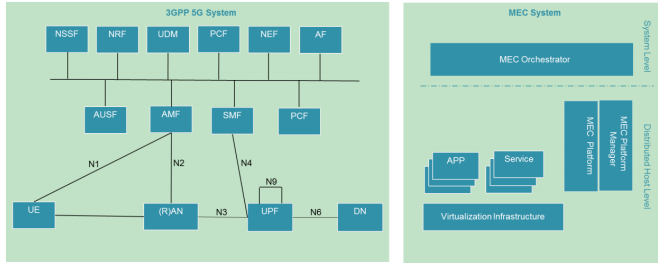
\includegraphics[width=\linewidth]{images/5GMEC-System-Architecture.png}
  \caption{5G Servicebasierte Architektur und MEC Systemarchitektur \cite{arnold5GRadioAccess2017} \cite{etsiETSIGSMEC}}
  \label{fig:sba}
\end{figure}
\\
Dieser Abschnitt beschreibt, wie ein Multi Access Edge Cloud System in die 5G-Netzwerkumgebung integriert werden kann 
und welche Komponenten miteinander iteragieren.
\\
\\
Die Netzwerkfunktionen und die Dienste die diese zur verfügungstellen, werden im 5G System in der Network Resource Funktion (NRF) registriert.
Bei dem NRF bietet damit eine Liste mit allen Diensten an. 
In einem MEC System werden die Dienste die von den MEC- Anwendungen bereitgestellt werden in der Service Registry in der MEC Platform registriert.
Will eine Netzwerkfunktion im 5G Netzwerk ein Dienst nutzen, kann diese direkt mit der Funktion die den Dienst zurverfügungstellt interagieren,
wenn diese au­then­ti­fi­zie­rt ist. Die Network Exposure Function (NEF) im 5G System stellt auch Dienste an nicht au­then­ti­fi­zie­rte Komponenten 
zur Verfügung. Die NEF ist damit sehr wichtig für die Bereitstellung von Servicen, sie ist verantwortlich für die Autorisierung aller Anfragen
auserhalb des 5G-Systems. 
\\
\\
Für die Integration von MEC in ein 5G Netzwerk, spielt die User Plane Function (UPF) eine wichtige Rolle. Die UPF ist Teil der User Plane
und ist eine Darstellung der dieser in Netzwerkfunktion. Die UPF ist das Gateway zur Kontrollen und Weiterleitung von Nutzdaten. \cite{Leitfaden5GCampusnetze2020}
Ist das MEC-System in die 5G Cloud integriert, ist die UPF auch Teil des MEC Systems.
\begin{figure}
  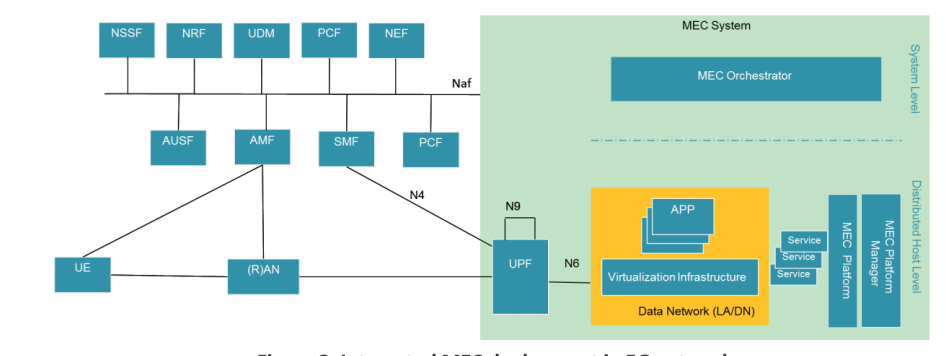
\includegraphics[width=\linewidth]{images/5GMEC-System-Architecture2.png}
  \caption{MEC in 5G}
  \label{fig:sba2}
\end{figure}
\\
In dem MEC- System auf der rechten Seite, agiert der MEC- Orchestartor auf der MEC- System Ebene. Dieser interagiert mit dem NEF oder
direkt mit den einzelnen Netzwerkfunktionen des 5G Netzwerks. Auf der MEC- Host Ebene, interagiert die MEC- Platform mit den NF des 5G Netzwerkes.
Die MEC- Host Ebene sind meistens in der UP des 5G Netzwerks, während der NEF als teil des CP als Systemlevel Funktion zentral eingesetzt wird.
Wie Abbildung \ref{fig:sba2} zeigt, befindet sich das MEC System auf der Data Control Ebene des 5G Netzwerkes. 
Die User Plane Function ist verantwortlich für das Weiterleiten der Datenpakete an die MEC zielanwendungen. 
Das MEC- System kann an verschiedenen Standorten in der nähe der Base Station des 5G Netzwerkes eingesetzt werden. 


\newpage
\section{Mobilitätsmanagement in Mobile Edge Clouds}
Die Mobilität von Endgeräte im 3GPP Neztwerken, kann dazu führen, dass ein UE sich von einer 
Radio Station zu nächsten bewegt. Das Verwalten und Aufrechterhalten dieser Verbindungen in Funknetzen wird
als Mobilitätsmanagement bezeichnet und ist eine Kernkomponenten von Funknezten. 
Wird eine aktive Funkverbindung von einer Netzwerkzelle zu einer anderen weitergegeben, wird der Vorgang
der Übergabe als Handoff oder Handover bezeichent.\\
Die Mobilität des Engeräges kann dazu führen, 
dass sich das UE zu einer anderen Zelle bewegt, 
die einem anderen MEC-Host zugeordnet ist. Dabei muss sichergestellt werden, dass der Netzwerkverkehr
richtig geroutet wird um das Ziel zu erreichen.
Entfernt sich das Engerät weiter vom Ort der MEC-Anwendung, 
kann dies dazu führen, dass die Latenz sich erhöht. Deshalb ist es wichtig, dass je nach Anwendung,
die laufende Anwendungsinstanz verschoben wird um die Latenz Anforderungen zu erfüllen. \\
Die Häufigkeit eines Wechsel der MEC Hosts, hängt stark von dem 
Einsatz ab. Bei der Verwendung von MEC für Autonomes Fahren treten häufiger Handover Envents ein, wie bei
beispielsweise Smart Factories.\\
Die Mobilität eines UEs kann in weitreichenden MEC-Systemen vorhergesagt werden und die einzelnen MEC-Host demnach konfiguriert werden,
dennoch muss der Zustand der Anwendung übertragen werden.
Dieses Kapitel beschreibt wie verschiedene Handoff Events ablaufen.

\subsection{Verschieben der Anwendung und desen Zustand}
Bewegt sich das UE im Funknetz und ist möglicherweise ein anderer Ziel MEC-Host geigneter als der aktuelle
MEC - Host, muss die Anwendung umziehen. Die MEC-Anwendungen werden in zustandslose und zustandsbehaftete Anwendungen eingeteilt.
Handelt es sich um eine zustandsbehaftete Anwendung, 
erfordert das Umziehen der Anwendung ein Synchronisieren des Zustands zwischen der aktuellen und der
verschobenen Anwendungsinstanz, um Kontinuität zu gewährleisten
muss auch umgezogen werden. 
\\
\\
Das Synchronisieren des Zustands muss bei dem Entwickeln der Anwendungen berücksichtigt werden. Diese muss so designt sein, 
dass die Anwendung in mehreren Instanzen auf unterschiedlichen MEC-Hosts betrieben werden kann. 
Für das Synchronisieren muss die Anwendungen das Feststellen des Zustands und kopieren dessens von einer Quell- Anwendung 
zu einer Zielanwendung unterstüzen. 
Läuft die Anwendung noch nicht auf dem Ziel Host, muss diese initalisiert und gestartet werden.
Nachdem die Anwendung gestartet ist, startet der Umzugsvorgang und der Zustand wird von dem aktuellen 
Host zu dem Ziel MEC-Host übertragen. Wenn der Zustand vollständig übertragen ist, stoppt die aktuelle Instanz
und die Ziel Instanz übernimmt das kommunizieren mit dem Endgerät.
\\
Für das Erkennen von UE Mobilität zu einer neuen Zelle, abboniert die MEC Platfor Radio Network Infromationen die von dem RNIS zu
Verfügung gestellt werden. Mithilfe dieser Informationen können UEs identifizieren werden bei denen eine Zelländerung auftritt 
und bestimmen werden, ob sie aus dem Versorgungsbereich des aktuellen MEC-Hosts herausbewegen.
TODO -> RNIS
\subsection{VM Handoff}
Eine vorgeschlagene Möglichkeit \cite{etsiETSIGSMEC} für das Umziehen laufenden Anwendungen von einem MEC-Host zu einem Ziel MEC-Host, 
ist der VM Handoff.  \cite{Ha2015AdaptiveVH}
\subsection{MEC Service Orchestrierung}
\label{subsec:MEC Service Orchestrierung}
\subsection{MEC Mobilität}
\label{subsec:MEC Mobilität}
\subsection{MEC Deployment}
\label{subsec:MEC Deployment}


\section{Anwendungen}
\label{sec:Anwendungen}
\subsection{Internet of Things}
\label{subsec:Internet of Things}
\subsection{Smart Factories}
\label{subsec:Smart Factory}
\subsection{Autonomes Fahren}
\label{subsec:Autonomes Fahren}
\section{Fazit und Ausblick}
Multi Access Edge Cloud Computing ist eine neue Technologie, die die Vorteile von
Edge Clouds und 5G optimial kombiniert und eine neue Platform zur Verfügung stellt.
MEC ist ist eine der wichtigsten neuen Technologien für 5G-Systeme, 
da es zur einer geringen Latenz und zur Kapazitätsverbesserung im Backhaul- und Kernnetzwerk führt. 
Der Erfolg von MEC hängt im Wesentlichen von der Ausrichtung der Technologie auf ETSI NFV ISG ab.
\subsection{Fazit}
\subsection{Ausblick}
Neben dem Ausbau des 5G Netzes, ist bei der Einführung von \textit{MEC} Systemen, 
die Standardisierung sehr wichtig. 
\subsection{Angebote}
\label{subsec:Angebote}
\label{sec:Ausblick}

% -------------------------------------------------------------------------------------------------

% -------------------------------------------------------------------------------------------------
\newpage
% Normaler LNCS Zitierstil
%\bibliographystyle{splncs}
\printbibliography[heading=bibintoc]


\end{document}
